\chapter{Python Bibliotheken}

Für Python gibt es Bibliotheken zum Laden von Daten, Visualisieren, Berechnen von Statistiken, Sprachverarbeitung, Bildverarbeitung usw. Dies gibt Data Scientists einen sehr umfangreichen Werkzeugkasten mit Funktionalität für allgemeine und besondere Einsatzgebiete, \cite{Mueller:2017}.
Numpy ist das Modul der Wahl, wenn man wissenschaftlich rechnen möchte und wird insbesondere für statistische Auswertungen, für Machine-Learning und allgemein für sehr aufwändige Berechnungen eingesetzt. Auf Numpy setzt unter Anderem auch TensorFlow, pandas, scipy, scikit-learn auf, \cite{Häberlein:2024}.

\section{Numpy}
NumericalPython, kurz NumPy, bietet Datenstrukturen und Algorithmen speziell für wissenschaftliche Anwendungen, \cite{McKinney:2023}. Grund hierfür ist, dass die Berechnung bei großen Daten-Arrays besonders effizient ist und somit schneller als normaler Python Code sein kann, \cite{McKinney:2023}. \\
Viele weitere Bibliotheken wie Pandas bauen auf NumPy auf, \cite{VanderPlas:2023}. Weitere Informationen der einzelnen Module können aus der NumPy Dokumentation entnommen werden, \cite{NumPy}

\section{Pandas}
 Pandas ist eine neuere Bibliothek und findet in der DataScience hohe Anwendung.  Sie bietet eine komfortable Schnittstelle zum speichern von Daten sowie eine Vielzahl an nützlicher Operationen. Die drei wichtigsten Datenstrukturen sind \textit{Series}, \textit{Index} und \textit{DataFrames}, \cite{VanderPlas:2023}.\\
 Ein DataFrame ist eine zweidimensionale, potenziell heterogene tabellarische Datenstruktur mit beschrifteten Achsen (Zeilen und Spalten). Diese entsprechen einem Zeilen- sowie Spaltenindex. Es kann als eine Art Container für Series-Objekte betrachtet werden, ähnlich wie ein Wörterbuch, das Spaltennamen als Schlüssel und Series-Objekte als Werte enthält. Ein DataFrame kann aus verschiedenen Datenquellen wie Listen, Dictionaries oder anderen DataFrames erstellt werden. Es bietet eine Vielzahl von Funktionen zur Datenmanipulation und -analyse und ist besonders nützlich für Aufgaben im Bereich der Datenanalyse. Pandas DataFrames können beispielsweise aus CSV-Dateien, Excel-Dateien oder SQL-Datenbanken eingelesen werden, \cite{VanderPlas:2023}. \\
 Beispielsweise kann ein Datensatz der Form 
 \begin{table}[H]
 	\small
 	\centering
 	\begin{tabular}{p{1.5cm}|p{1.5cm}|p{1.5cm}|p{1.5cm}|p{1.5cm}}
 		$x$ & $y_1$ & $y_2$ & $y_3$ & $y_4$ \\ \hline
 		-20.0 & 100.21 & -19.75 & 0.34 & 19.77 \\
 		-19.9 & 99.89 & -19.70 & 0.61 & 19.78 \\
 		-19.8 & 99.39 & -19.56 & 0.17 & 19.44 \\
 		-19.7 & 98.24 & -19.85 & 0.73 & 19.86 \\
 	\end{tabular}
 	\caption{Beispiel Panda DataFrame}
 	\label{tab:Pandas DF}
 \end{table}
 folgendermaßen
 \begin{lstlisting}[caption={Pandas Dataframe}, captionpos=b, label={lst:Dataframe}]
	data = 
	{
		'x': [-20.0, -19.9, -19.8, -19.7],
		'y1': [100.216064, 99.894684, 99.397385, 98.24446],
		'y2': [-19.757296, -19.70282, -19.564255, -19.858267],
		'y3': [0.3461139, 0.61786354, 0.1743704, 0.7310719],
		'y4': [19.776287, 19.789793, 19.441765, 19.869267]
	}
	df = pd.DataFrame(data)
 \end{lstlisting}
 in ein Dataframe geschrieben werden. Dieses DataFrame hat den Spaltenindex \textit{'x', 'y1', y2', 'y3', 'y4'}, abrufbar über \textit{df.columns}, sowie den Zeilenindex \textit{'0', '1', '2', '3'}, abrufbar über \textit{df.index}.\\
 
 In der Klasse \textit{Data} aus Kapitel \ref{lst:class data} wird mittels der Pandas Funktion
 \begin{lstlisting}
 	self.df = pd.read_csv(datapath)
 \end{lstlisting}
 eine .csv Datei eingelesen und als DataFrame gespeichert. 
 Weitere nützliche Funktionen sind die \textit{df.sort} Funktion
 \begin{lstlisting}
 	self.dfSortByX = self.df.sort_values(['x'])
 \end{lstlisting}
 welche das DataFrame anhand der x-Spalte sortiert.
 
 \section{Bokeh}
 Bokeh ist eine interaktive Datenvisualisierungsbibliothek für Python, die sich dadurch auszeichnet, umfassende interaktive Grafiken zu erstellen. Sie ist kompatibel mit Webtechnologien wie HTML, CSS und JavaScript und kann auf verschiedenen Plattformen wie Jupyter Notebook, JupyterLab, Flask und Django eingesetzt werden.
 Sie bietet eine breite Palette von Diagrammtypen, darunter Linien-, Streu-, Balken-, Flächen-, Histogramme- und zahlreiche weitere Diagramme. Bokeh zeichnet sich durch seine Schnelligkeit bei der Arbeit mit großen Datensätzen aus und ermöglicht es Nutzern, Grafiken anzupassen und interaktiv zu betrachten. 
 
Abbbildung \ref{fig:bokeh} dient beispielhaft für die Erstellung eines Plots mittels Bokeh. Diese wurde mit dem \textit{scatter}- Befehl erstellt und verarbeitet die \textit{x} und \textit{y} werte eines Pandas \textit{DataFrame}.
 \begin{figure}[h]
 	\centering
 	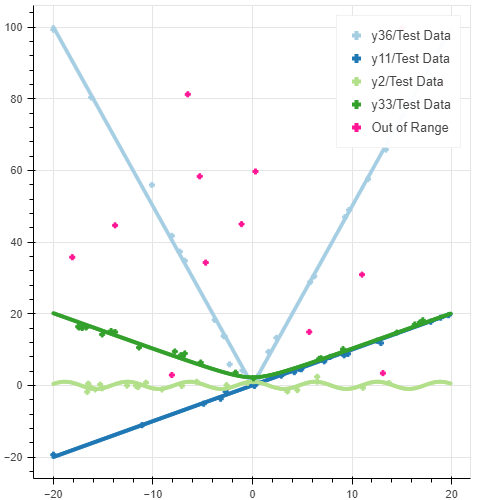
\includegraphics[width=8cm]{pics/bokeh_plot.png}
 	\caption{Beispiel eines Plots mit Bokeh }
 	\label{fig:bokeh}
 \end{figure} 
 
 \begin{lstlisting}[caption={Bsp.: Bokeh Scatter-Plot}, captionpos=b, label={lst:plot}]
 	ax.scatter(idFcnsDf['x'].values, idFcnsDf['y'].values,size=3,
 		color=colors[i])
 \end{lstlisting}
 
 Müssen mehrere Farben verwendet werden, bietet Bokeh eine breite Auswahl an Farbpaletten. Abbildung \ref{fig:bokeh} wurde mit der \textit{brewer paired} Farbpalette erstellt. 
 \begin{lstlisting}[caption={Bokeh Farb-Palette}, captionpos=b, label={lst:brewer color}]
 	colors = palettes.brewer['Paired'][4]   
 \end{lstlisting}
 